\documentclass{article}
\usepackage{graphicx} % Required for inserting images

\title{phys-ga-2000-ps6}
\author{knd286 }
\date{October 2024}

\begin{document}

\maketitle

\section{Part a}
Plotting a handful of galaxies, a common feature I see is a peak between 600 and 700nm. This  corresponds to the transition from $E_2$ to $E_3$ in a hydrogen atom. You can see the random handful of galaxies i plotted in figure 1.
\begin{figure}[h!]
    \centering
    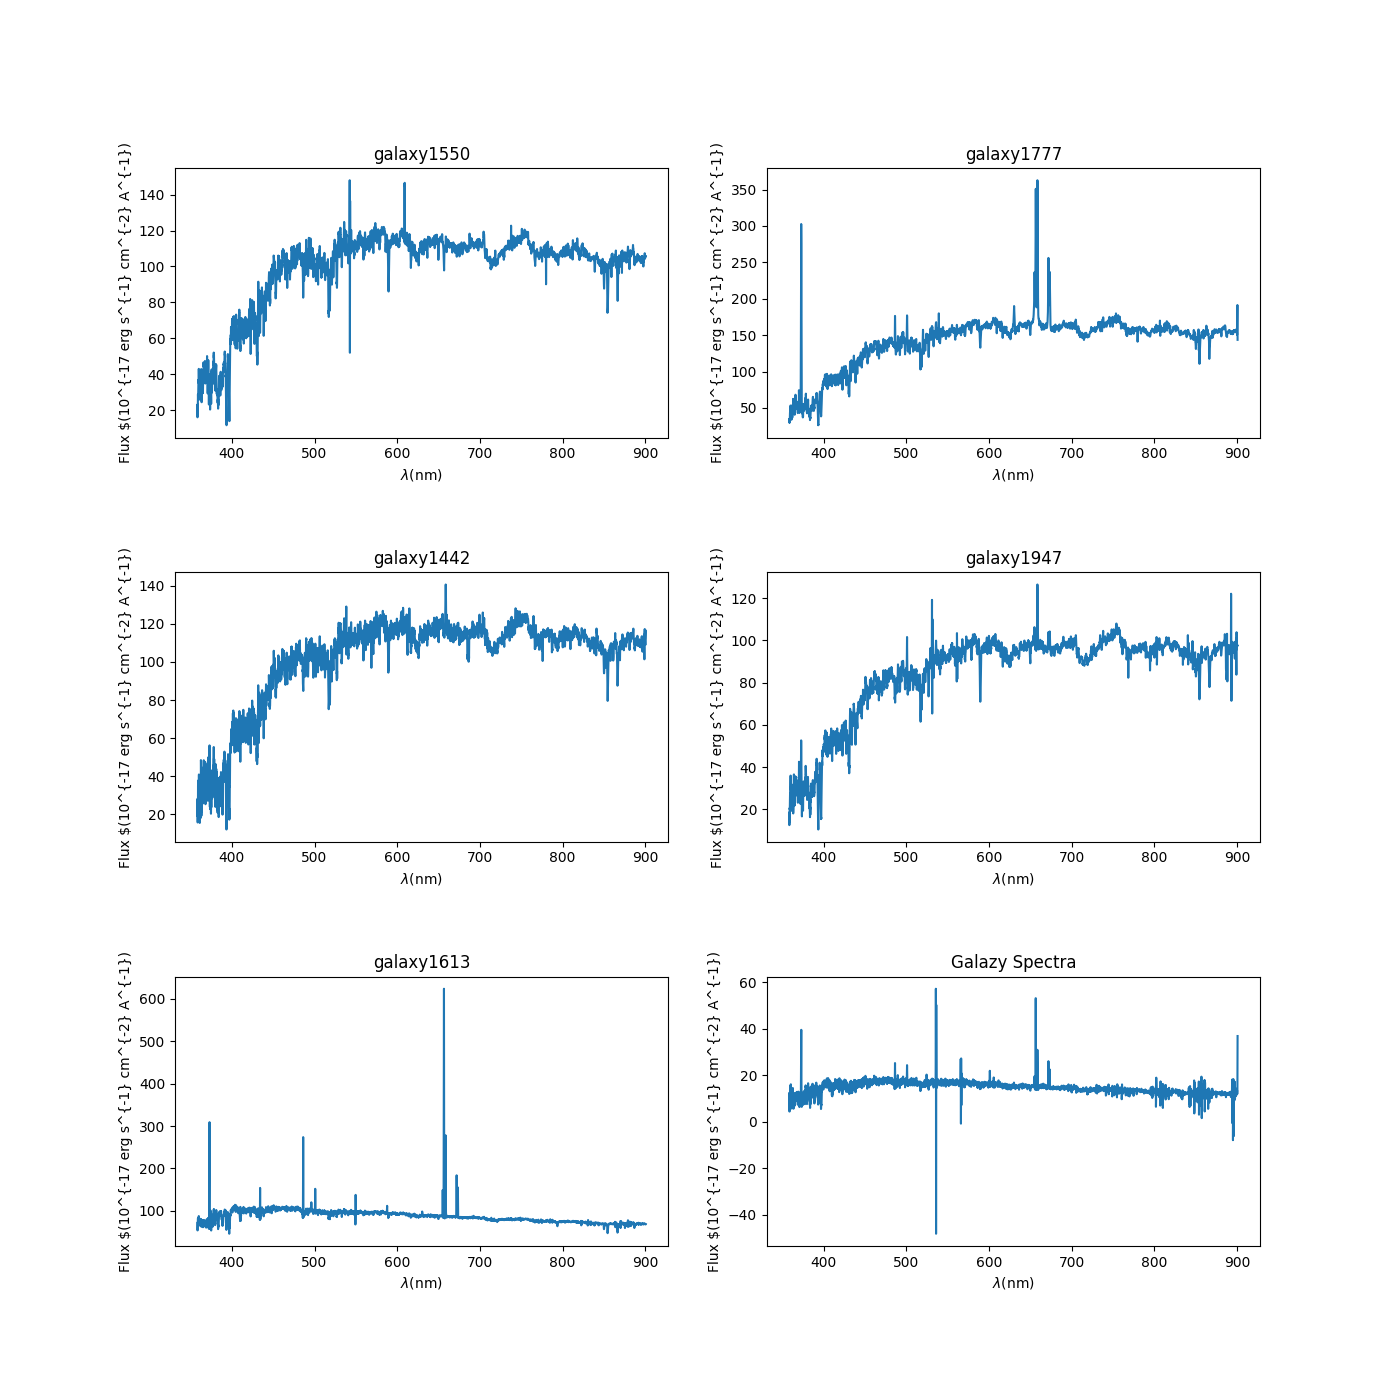
\includegraphics[width=0.8\linewidth]{partA.png}
    \caption{The spectrum of a few random galaxies}
    \label{The flux of a few random galaxies}
\end{figure}
\section{Part d}
I followed the steps outlined in the homework and found the covariance matrix. I used the function np.linalg.diag() to find the eigenvectors and eigenvalues of C. In figure 2, you can see a plot of the first 5 eigenvectors of the covariance matrix

\begin{figure}[h!]
    \centering
    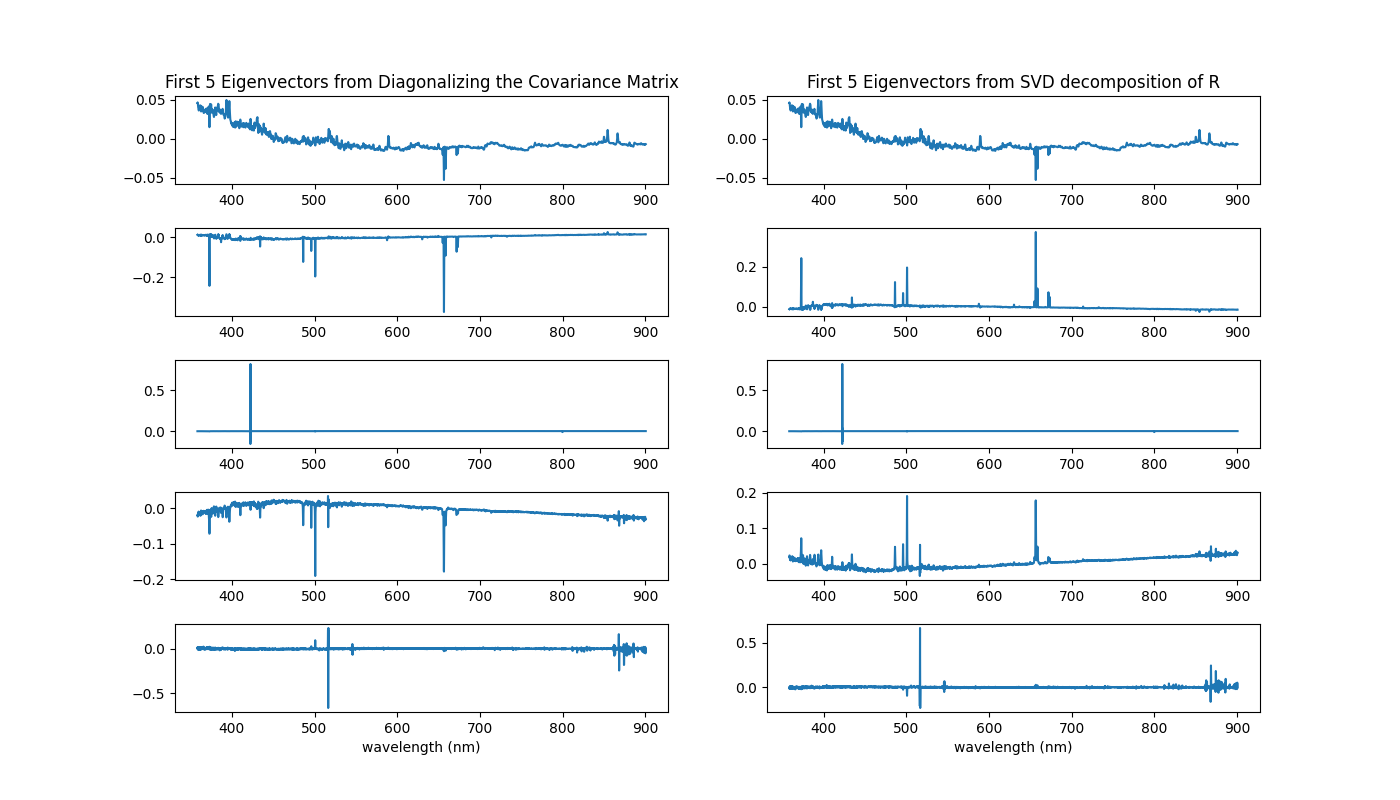
\includegraphics[width=0.8\linewidth]{first_5_eigen_vec.png}
    \caption{First 5 Eigenvectors}
    \label{fig:enter-label}
\end{figure}

\section{Part e}
I then used SVD on the matrix "R", to find the eigenvectors and eigenvalues of C. You can see the first 5 eigenvectors found from using this method plotted in figure 2. They appear equivalent. Some of the eigenvectors are scaled by -1, but that is ok.
\par


\section{part f}
The condition number of R  is: 4685956010237581.0. The condition number of C is 2.208895086648627e+18. It is much faster to perform SVD on R then it is to diagonalize C.

\section{part g}
To approximate the spectrum with the first 5 eigenvectors, first I projected on to first 5 eigen basisi vectors, then using that projection, I reconstructed the spectrum. here is what the first 5 spectra looked like when reconstructed from the first 5 eigenvectors. 
\begin{figure}[h!]
     \centering
     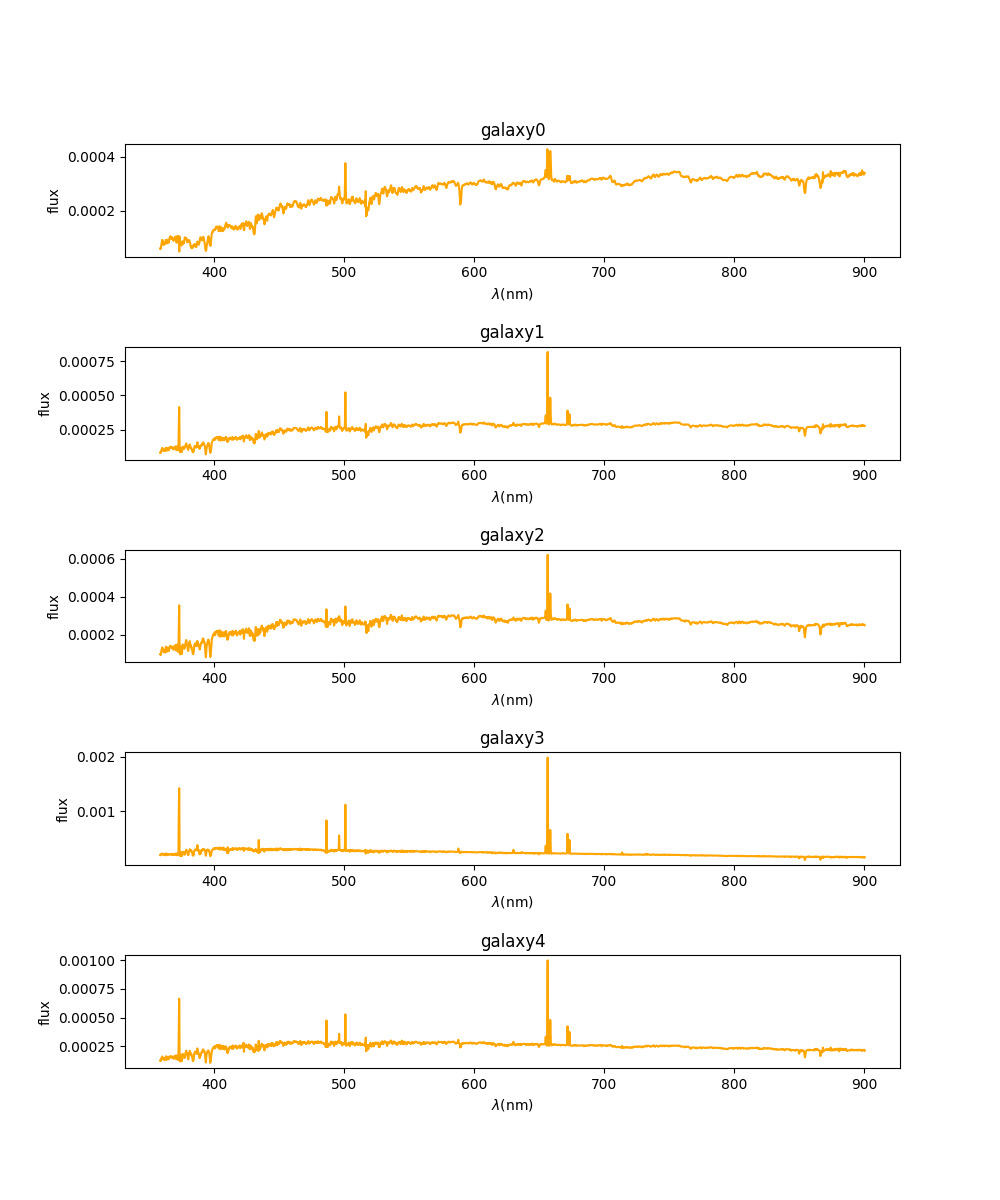
\includegraphics[width=0.8\linewidth]{approxSpectra5.png}
     \caption{Reconstructed Spectrum}
     \label{fig:enter-label}
 \end{figure}


\section{part h}

fig 4 has a plot of C0 vs c1 and c0 vs c2
\begin{figure}[h!]
    \centering
    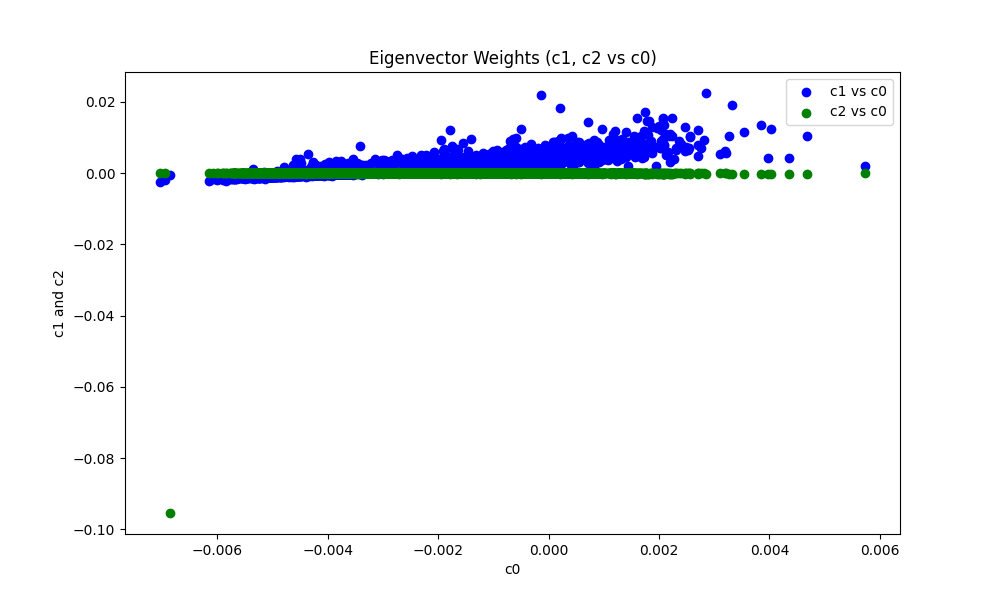
\includegraphics[width=0.8\linewidth]{c0vc1.png}
    \caption{c0 vs c1}
    \label{fig:enter-label}
\end{figure}

\section{part i}
fig 4 shows how the error between the reconstructed spectra and the actual spectra decreases as you add more eigenvectors into the approximation.

\begin{figure}
    \centering
    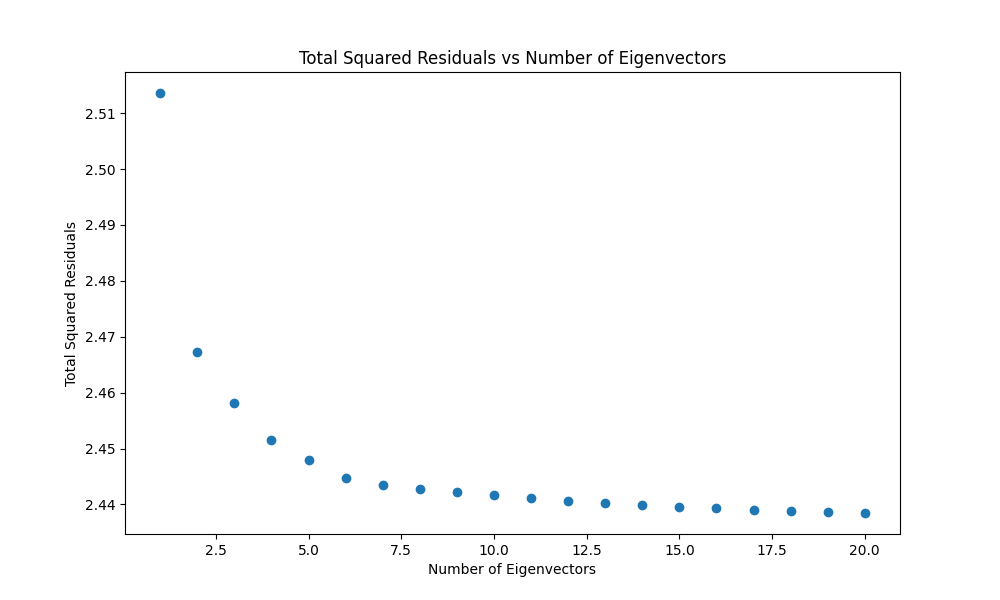
\includegraphics[width=0.8\linewidth]{residuals_v_Nc.png}
    \caption{Residuals vs Number}
    \label{fig:enter-label}
\end{figure}
\end{document}
